\documentclass{beamer}
\usetheme{AnnArbor}
\usecolortheme{beaver}
\usepackage[utf8]{inputenc}
\usepackage[T1]{fontenc}
\usepackage[italian]{babel}
\usepackage{soul}
\usepackage{graphicx}
\usepackage{algorithm2e}
\usepackage{multirow}

\usepackage{fancyvrb}
\definecolor{felinesrcbgcolor}{rgb}{1,1,0.85}
\definecolor{felinesrcbgcolor}{rgb}{0.94,0.97,1}
\definecolor{felineframe}{rgb}{0.79,0.88,1}
\definecolor{myorange}{rgb}{1,0.375,0}
\fvset{frame=lines,
  framesep=3mm,
  framerule=3pt,
  fontsize=\small,
  rulecolor=\color{myorange},
  formatcom=\color{DarkGreen},
}

\hypersetup{
	urlcolor=myorange
}

\title[Arch2013] % (optional, only for long titles)
{Architettura degli elaboratori 2012/2013}
\subtitle{Aritmetica binaria: Signed, Fixed e Float}
\author{Michele ``Jazzinghen'' Bianchi\inst{1}}
\institute[DISI] % (optional)
{
  \inst{1}%
  Dipartimento di Ingegneria e Scienze dell'Informazione\\
  Universtià degli Studi di Trento
}
\date[2013-03-06] % (optional)
{06 Marzo 2013}
\subject{Computer Science, Embedded Systems}

\begin{document}
	\frame{\titlepage}
	\section{It's answer TIME!}
	\begin{frame}
    \frametitle{Alcune cose prima d'iniziare}
    \framesubtitle{Ve l'avevo detto che avrei risposto}
		\begin{itemize}
			\item La t-shirt che indossavo l'altra volta era di Think Geek: \url{http://www.thinkgeek.com/product/dae9/}\footnote{Quella
				di oggi è di \url{http://www.redbubble.com/}}
			\item Il mio sito web (quello con sopra la roba) è: \url{http://disi.unitn.it/~bianchi}. È fatto con
				jQuery, PHP, HTML5 e CSS3.
			\item La parte in assembly verrà fatta usando l'X86\_64.
			\item GCC bara! La somma tra uint{8,16,32,64} ed int viene fatta attraverso magheggiamenti\footnote{Dettagli sul sito}!
		\end{itemize}
	\end{frame}   
   
  \section[Being negative]{Interi con il segno}
	\subsection{Riassunto dell'ultima puntata}  
  \begin{frame}
    \frametitle{Cos'è successo l'ultima volta?}
		Abbiamo visto:    
    \begin{itemize}
    		\item Come sono stati rappresentati i numeri durante le ere
    		\item Le varie strutture dati utilizzate dai computer
    		\item Come passare da base-2 a base-10 ed il contrario
    		\item L'aritmetica con i Naturali binari
    		\item Come aggiungere il segno ai numeri binari
    \end{itemize}
    %Unari, Babilonesi, Romani, Posizioniali (indiani), Binaria
  \end{frame}
	
	\subsection{Somma / Sottrazione}
  \begin{frame}
    \frametitle{Interi con il segno}
    \framesubtitle{Somma e Sottrazione}
    Le due operazioni sono la stessa cosa!
    
		\vspace{2em}    
    
    Grazie alla convenzione usata (Complemento-2) basta sommare due numeri signed, 
    ignorando il bit di overflow, per avere il risultato.
  \end{frame}
  
  \begin{frame}
	    \frametitle{Somma e Sottrazione di interi}
	    \framesubtitle{Esempio}
	    $$117_{10} - 34_{10} = 01110101_{2} + 11011110_{2} = \text{?}$$
	    \vspace{2em}
	    \pause
			\begin{center}
			\begin{tabular}{cccccccc|c} 
			 0 & 1 & 1 & 1 & 0 & 1 & 0 & 1 & + \\  
			 1 & 1 & 0 & 1 & 1 & 1 & 1 & 0 & = \\ 
			\hline 
			 0 & 1 & 0 & 1 & 0 & 0 & 1 & 1 &  \\ 
			\end{tabular}
			\end{center}
			\pause
			\vspace{2em}
			$$01010011_{2} = 83_{10}$$
	  \end{frame}

	\subsection{Moltiplicazione signed}  
  \begin{frame}
    \frametitle{Moltiplicazione signed: Algoritmo di Booth}    	
		Possiamo moltiplicare i signed come facevamo con gli unsigned,
		solo che questo può richiedere una quantità di tempo impressionante.
		
		\vspace{2em}
		
		È per questo che utilizziamo un metodo creato da Andrew Donald Booth, che studiava,
		ovviamente, cristallografia.
		
		\vspace{2em}
		
		Il processo utilizza un concetto molto semplice, ovvero che:
		
		$$01\text{...}1 = 10\text{...}0 - 1$$
  \end{frame}
  \begin{frame}
    \frametitle{Moltiplicazione signed: Algoritmo di Booth}
    \framesubtitle{L'algoritmo di Booth}
    \begin{columns}
    \column{.5\textwidth}
    	  L'algoritmo è molto semplice.
    	  
    	  Si tratta di scorrere le cifre del secondo termine del
    	  prodotto e guardare la cifra immediatamente a destra
    	  (la prima cifra a destra è sempre 0).
    	  
			\vspace{2em}    	  
    	  
    	  In base a quale è la coppia bisognerà sommare o sottrarre
    	  il primo termine del prodotto.
    \column{.5\textwidth}
    		\begin{center}
			\begin{tabular}{|c||p{6em}|}
				\hline				
				Coppia di valori & Operazione \\
				\hline
				00 & \multirow{2}{*}{Nulla} \\
				11 & \\
				\hline				
				10 & Sottrare il moltiplicando 	\\
				\hline				
				01 & Sommare il motiplicando 		\\
				\hline 
			\end{tabular}
			\end{center}
    \end{columns}
  \end{frame}

  \begin{frame}
    \frametitle{Moltiplicazione signed: Algoritmo di Booth}
    \framesubtitle{Esempio}
    
  \end{frame} 
  
  \section[Fixed]{Numeri binari frazionari}
  \begin{frame}
  		\frametitle{Un test}
  		Ok, quanto è $11101.01001_{2}$ in base-10? (solo positivo)
  		
  		\vspace{2em}
    \pause
		\begin{center}
		\begin{tabular}{ccccccccccc} 
		 $2^4$ & $2^3$ & $2^2$ & $2^1$ & $2^0$ & . & $2^{-1}$ & $2^{-2}$ & $2^{-3}$ & $2^{-4}$ & $2^{-5}$ \\		 
		 1 & 1 & 1 & 0 & 1 & . & 0 & 1 & 0 & 0 & 1 \\ 
		\hline 
		 16 & 8 & 4 & 0 & 1 & . & 0 & $1/4$ & 0 & 0 & $1/32$ \\ 
		\end{tabular}
		\end{center}
		\pause
		\vspace{2em}
		
		$$11101.01001_{2} = 29_{10} + \frac{9}{32}_{10} = 29.28125_{10} $$
  		
  \end{frame}
  \begin{frame}
  		\frametitle{Numeri binari frazionari: Fixed Point}
  		Funzionano come i numeri interi, solo che la parte a destra del "punto binario" è formata
  		da potenze frazionarie di due (i.e. potenze negative di 2).
  		
  		\vspace{2em}
  		
  	  Tutte le operazioni sono come quelle che abbiamo visto per gli interi (somma, sottrazione, moltiplicazione, shifting)
  	  
  	  \vspace{2em}
  	  
  	  \begin{block}{Utilizzo fixed Point}
  	  		Questa rappresentazione dei numeri viene utilizzata su sistemi che non dispongono di una Floating
  	  		Point Unit (FPU). Una volta erano molto più utilizzati. Tipo nella PS1, nel Saturn, nel GBA, nel
  	  		Nintendo DS... NEL SATURN! Vuol dire che il Dreamcast aveva già una FPU (anzi 4)
  	  \end{block}
    
  \end{frame}
  \subsection{Limiti}
	\begin{frame}
    \frametitle{Fixed Point}
    \framesubtitle{Limiti}
    \begin{itemize}
			\item Pochi linguaggi hanno un supporto built-in dei Fixed (C e C++ ce l'hanno grazie a GCC)
    		\item Possono rappresentare solo numeri nella forma $\frac{k}{2^x}$
    		\item Tutti gli altri numeri razionali si possono rappresentare
    			solo usando una serie di bit decimali periodica.
    \end{itemize}
    \vspace{1em}
    $$\frac{1}{3}_{10} = 0.\overline{01}_{2}$$
    $$\frac{1}{5}_{10} = 0.\overline{0011}_{2}$$
    $$\frac{1}{10}_{10} = 0.0\overline{0011}_{2}$$
  \end{frame}
  \begin{frame}
    \frametitle{Conversione base-10 a base-2}
    \framesubtitle{Divisione e modulo}
    \begin{itemize}
    		\item Più facilmente implementabile
    \end{itemize}
    \begin{columns}
    \column{.6\textwidth}
    \footnotesize{
    \begin{algorithm}[H]
    		\SetAlgoLined
			 \KwData{n: Numero base-10 da convertire}
			 \KwResult{s: Numero convertito in base-2}
			 s = stringa vuota\;			 
			 \While{n>0}{
			  s = (n mod 2) + s\; 
			  n = n div 2\;
			 }
    \end{algorithm}
		}
	  \column{.4\textwidth}
	 	\footnotesize{		
			\pause
	 		$$97_{10} = ??$$
		  \pause
			\begin{tabular}{|c|l|}
			\hline
			 n & s \\
			\hline
	     97 & \\
	     48 & 1 \\
	     24 & 01 \\
	     12 & 001 \\
	     6 & 0001 \\
	     3 & 00001 \\
	     1 & 100001 \\
	     0 & 1100001 \\
			\hline
			\end{tabular}
		  $$97_{10} = 1100001_{2}$$ 
		}		
	  \end{columns}
		
		
  \end{frame}
  \begin{frame}
    \frametitle{Conversione base-10 a base-2}
    \framesubtitle{Sottrazione}
    \begin{itemize}
    		\item Terribile se usato con numeri grandi
    \end{itemize}
	\begin{columns}
  \column{.6\textwidth}
    \footnotesize{
    \begin{algorithm}[H]
    		\SetAlgoLined
			 \KwData{n: Numero base-10 da convertire}
			 \KwResult{s: Numero convertito in base-2}
			 s = stringa vuota\;
			 i = massima potenza di due contenuta in n\;		 
			 \Repeat{i=0}{
			  \eIf{$i \leq n$}{
			  		s = s + ``1''\; 
			  		n = n - i\;
			 }{
			 		s = s + ``0''\;
			 }
			  i = i div 2\;
			 }
    \end{algorithm}
	}
  \column{.4\textwidth}
 	\footnotesize{		
		\pause
 		$$117_{10} = ??$$
	  \pause
		\begin{tabular}{|c|c|l|}
		\hline
		 n & i & s \\
		\hline
     117 & 64 & \\
     53 & 32 & 1 \\
     21 & 16 & 11 \\
     5 & 8 & 111 \\
     5 & 4 & 1110 \\
     1 & 2 & 11101 \\
     1 & 1 & 111010 \\
     0 & 0 & 1110101 \\
		\hline
		\end{tabular}
	  $$117_{10} = 1110101_{2}$$ 
	}		
  \end{columns}
  \end{frame}
  
  \section[Operations]{Aritmetica dei naturali}
	\subsection[NatSum]{Somma di Naturali}  
	  \begin{frame}
	    \frametitle{Somma di naturali}
	    \framesubtitle{Un'introduzione, prima}
			\begin{center}
	    \begin{tabular}{|c|c|c||c|c|}
	    		\hline
	    			A & B & Carry & C & Carry \\
	    		\hline
	    			0 & 0 & 0 & 0 & 0 \\
	    			1 & 0 & 0 & 1 & 0 \\
	    			0 & 1 & 0 & 1 & 0 \\
	    			1 & 1 & 0 & 0 & 1 \\
	    			0 & 0 & 1 & 1 & 0 \\
	    			1 & 0 & 1 & 0 & 1 \\
	    			0 & 1 & 1 & 0 & 1 \\
	    			1 & 1 & 1 & 1 & 1 \\
	    		\hline
	    \end{tabular}
	    
	    \vspace{2em}
	    
	    A + B + Carry = C + Carry
	    \end{center}	  
	  \end{frame}
	  \begin{frame}
	    \frametitle{Somma di naturali}
	    \framesubtitle{Esempio}
	    $$117_{10} + 97_{10} = 1110101_{2} + 1100001_{2} = \text{?}$$
	    \vspace{2em}
	    \pause
			\begin{center}
			\begin{tabular}{cccccccc|c} 
			 & 1 & 1 & 1 & 0 & 1 & 0 & 1 & + \\  
			 & 1 & 1 & 0 & 0 & 0 & 0 & 1 & = \\ 
			\hline 
			1 & 1 & 0 & 1 & 0 & 1 & 1 & 0 &  \\ 
			\end{tabular}
			\end{center}
			\pause
			\vspace{2em}
			$$11010110_{2} = 214_{10}$$
	  \end{frame}
  \subsection[NatSub]{Sottrazione di Naturali}  
	  \begin{frame}
	    \frametitle{Sottrazione di naturali}
	    \framesubtitle{Operazione di base e ``Il prestito''}
	    Come nella somma si va da destra a sinistra seguendo delle regole banali:
			
			\vspace{2em}	    
	    
	    \begin{center}
		    \begin{tabular}{|c||c|c|c|c|}
		    \hline 
		    A & 0 & 1 & 1 & \textbf{0} \\ 
		    \hline 
		    B & 0 & 0 & 1 & \textbf{1} \\ 
		    \hline 
		    A-B & 0 & 1 & 0 & \textbf{1} \\ 
		    \hline 
		    \end{tabular}
	    \end{center}
	    
	    \vspace{2em}
	    
	    Nell'ultimo caso bisogna scorrere a sinistra finchè
	    non si trova un 1, invertendo il valore di tutte le cifre incontrate, 1 compreso.
	    
	    $$ 10..0 \rightarrow 01..1 $$
	  \end{frame}
	  \begin{frame}
	    \frametitle{Sottrazione di naturali}
	    \framesubtitle{Esempio}
	    $$214_{10} - 117_{10} = 11010110_{2} - 1110101_{2} = \text{?}$$
	    \vspace{2em}
	    \pause
			\begin{center}
			\begin{tabular}{cccccccc|c} 
				1 & 1 & 0 & 1 & 0 & 1 & 1 & 0 &	- \\		 
			 		& 1 & 1 & 1 & 0 & 1 & 0 & 1 & = \\  
			\hline			 
			 & 1 & 1 & 0 & 0 & 0 & 0 & 1 &  \\ 
			\end{tabular}
			\end{center}
			\pause
			\vspace{2em}
			$$1100001_{2} = 97_{10}$$
	  \end{frame}
	\subsection[NatMul]{Moltiplicazione di Naturali}  
	  \begin{frame}
	    \frametitle{Moltiplicazione di naturali}
	    \framesubtitle{Moltiplicazione (e divisione) per potenze di due}
	    Ok, se dobbiamo moltiplicare un numero base-10 per 10 dobbiamo...
	    
	    \pause
	    
	    \begin{center}
		    Aggiungere uno 0 a destra.
		    
		    
\includegraphics[width=.5\textwidth]{IMGs/youdontsay.png}
	    \end{center}
	    
	  \end{frame}
	  \begin{frame}
	    \frametitle{Moltiplicazione di naturali}
	    \framesubtitle{Moltiplicazione (e divisione) per potenze di due, cont.}
	    Nel caso dei numeri base-2, aggiungere uno 0 a destra significa
	    moltiplicare il numero per 2, mentre eliminando la prima cifra a
	    desra significa dividere per 2.
	    
	    \vspace{2em}
	    
	    Questa operazione è chiamata shifting, utilizzata spesso dai compilatori
	    per ottimizzare la moltiplicazione.
	  \end{frame}
	  \begin{frame}
	    \frametitle{Moltiplicazione di naturali}
	    \framesubtitle{Moltiplicazione tra due Naturali}
	    Moltiplicare due numeri base-2 naturali altro non è che l'applicazione
	    di shifting multipli e poi della somma sui risultati degli shifting.
	    
	    \vspace{2em}
	    
	    Alla fine non è differente dalla moltiplicazione in base-10, solo che è più
	    semplice perché o bisogna sommare uno dei due moltiplicatori shiftati o nulla.
	  \end{frame}
		\begin{frame}
	    \frametitle{Moltiplicazione di naturali}
	    \framesubtitle{Esempio}
			
			$$13_{10} x 17_{10} = 1101_{2} x 10001_{2} = \text{?}$$
	    \vspace{1em}
	    \pause	    
	    \begin{center}
	    \begin{tabular}{cccccccc||c}
	      &   &   &   & 1 & 1 & 0 & 1 & x \\ 
	      &   &   & 1 & 0 & 0 & 0 & 1 & = \\ 
	    \hline 
	      &   &   &   & 1 & 1 & 0 & 1 &  + \\ 
	      &   &   &   &   &   & - &   &  + \\ 
	      &   &   &   &   & - &   &   &  + \\ 
	      &   &   &   & - &   &   &   &  + \\ 
	    1 & 1 & 0 & 1 &   &   &   &   &   \\ 
	    \hline 
	    1 & 1 & 0 & 1 & 1 & 1 & 0 & 1 &   \\ 
	    \end{tabular} 
	    \end{center}
	    
	    \pause
			\vspace{1em}
			$$11011101_{2} = 221_{10}$$
	  \end{frame}
	\subsection[Errors]{Error checking}
		\begin{frame}
	    \frametitle{Error Checking}
	    \framesubtitle{Overflow/Underflow}
	    \begin{columns}
			\column{.6\textwidth}	    
			\footnotesize{
	    Fino ad ora abbiamo sempre fatto calcoli pensando di avere cifre infinite a nostra disposizone.
    
	    ...
	    
	    Purtroppo, la realtà ci impone dei limiti di spazio, dettati
	    dall'architettura di basso livello del calcolatore.
	    
	    A causa di questo si possono rischiare errori da semplicemente stupidi a catastrofici.
	    
	    \vspace{1em}
	    \pause
	    
	    Tipo quello che è successo all'Ariane 5 501, missile Geostationary Transfer Orbit (GTO), progettato
	    dalla Astrium per l'ESA. A causa di un errore di conversione e di mancato controllo degli Overflow
	    la casa di produzione ha bruciato 370M\$ in circa 40 secondi.
	    }
	    \column{.4\textwidth}
	    \begin{center}
	    		
\includegraphics[width=.9\textwidth]{IMGs/overflow.jpeg}
	    \end{center}
	    \end{columns}
	  \end{frame}
	  
	\begin{frame}
    \frametitle{Error Checking}
    \framesubtitle{Overflow/Underflow cont.}
    Possiamo immaginare i numeri in base-2 con una quantità limitata di cifre come se fossero posti
    intorno ad una ruota:
    
    \begin{center}
    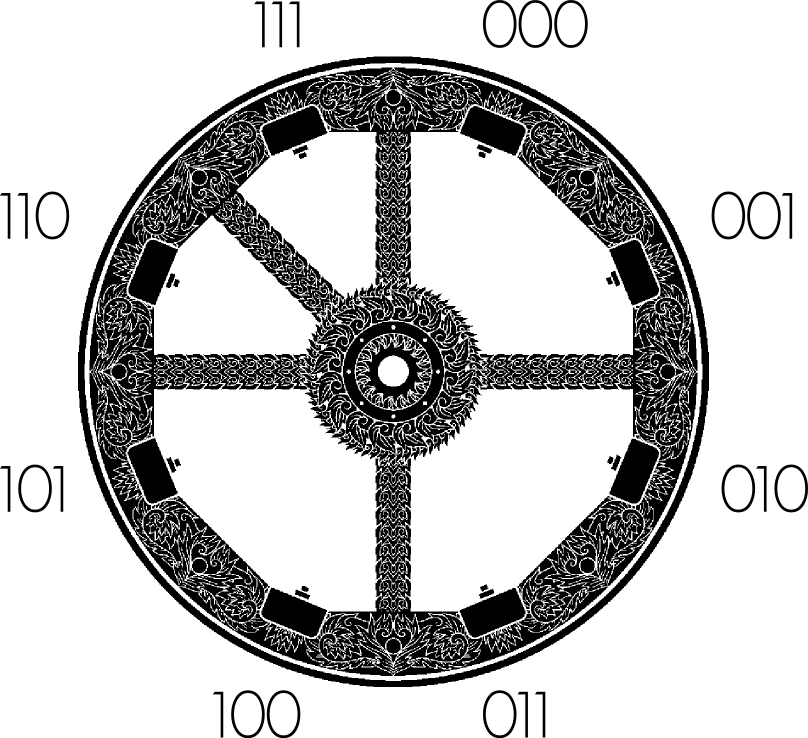
\includegraphics[width=.5\textwidth]{IMGs/TheBurningWheel.png}
    \end{center}

  \end{frame}
  
  	\begin{frame}
    \frametitle{Error Checking}
    \framesubtitle{Overflow/Underflow cont.}
    Nel caso precedente il numero è formato al massimo da 3 cifre binarie, quindi, se noi provassimo a
    calcolare $111_{2} + 1_{2}$ il risultato dovrebbe essere $1000_{2}$, solo che non abbiamo abbastanza
    cifre per contenere tutte le informazioni.
    
    Il risultato sarà quindi $000_{2}$. In pratica, $7_{10} + 1_{10} = 0_{10}$.
    
    \vspace{2em}
    \pause
    
    Fortunatamente le ALU contengono delle flag che indicano se è avvenuto un overflow (o un underflow)
    durante un'operazione aritmetica.
  \end{frame}
  
  \section[NegativeRep]{Aggiunta del segno negli interi}
  \begin{frame}
  		\frametitle{Aggiungere il segno agli interi}
  		Il supporto per i numeri negativi è stato aggiunto in vari modi\footnote{I quali dimezzano il
  		numero massimo rappresentabile}:
    \begin{itemize}
    		\item \emph{Segno-e-Modulo}: Un bit fa da segno, gli altri sono il valore del numero
    		\item \emph{Complemento ad 1}: Per avere il numero negativo invertiamo tutti i bit.
    		\item \emph{Complemento a 2}: Facciamo il complemento ad 1 e poi sommiamo 1.
    \end{itemize}
  \end{frame}
  \subsection{Segno-e-Modulo}
  \begin{frame}
  		\frametitle{Aggiungere il segno agli interi}
    \framesubtitle{Rappresentazione in Segno-e-Modulo}
    
    \begin{itemize}
    		\item Più vicino (Anzi, esattamente IL) al metodo usato per la rappresentazione dei negativi nei float
    		\item Permette l'esistenza di due 0: $+0$ e $-0$
    		\item Richiede una logica più complessa per venir implementato.
    \end{itemize}
  \end{frame}
  \subsection{Complemento a 2}
  \begin{frame}
  		\frametitle{Aggiungere il segno agli interi}
    \framesubtitle{Complemento a 2}
		Il complemento ad 1 è migliore del Segno-e-Modulo per gli interi, ma ha ancora dei problemi, tipo
		il doppio $0$ oppure il fatto che è macchinoso a causa dell'offset di $-1$ dei numeri negativi.
		
		Per questo è stato inventato il complemento a 2:
		
		\begin{itemize}
			\item Solo uno 0
			\item Trasparente per somma, sottrazione e moltiplicazione
			\item Per questo molto più facilmente implementabile a livello hardware
		\end{itemize}		    
    %Complemento ad 1 sarebbe figo, ma ci sega un valore. Complemento a 2 (Cmpl1 + 1) rimuove il problema. 
  \end{frame}
% etc
\end{document}
